
\documentclass[14pt]{article}
\usepackage{pgf}
\usepackage{underscore}
\usepackage{amssymb}
\usepackage{tabularx}
%\usepackage{fontspec}
%\usepackage{unicode-math}
\usepackage{color}
\usepackage{setspace}
\usepackage{hyperref}
\usepackage[table]{xcolor}
\usepackage[dvipsnames]{xcolor}
\usepackage{listings}
\usepackage[fontsize=14pt]{fontsize}
\onehalfspacing{}
\usepackage{cite}
\usepackage{amsmath}
\usepackage{amsfonts}
\usepackage{tikz}
\usepackage{graphicx}
\usetikzlibrary{automata, positioning, arrows}
%\setmainfont[Ligatures=TeX]{TeX Gyre Pagella}
%\setsansfont{TeX Gyre Heros}
%\setmonofont{TeX Gyre Cursor}
%\setmathfont{TeX Gyre Pagella Math}

\newcommand\given[1][]{\:#1\vert\:}
\DeclareMathOperator{\SPAN}{span}

% SHOW SOLUTION
%\renewcommand{\solutiontitle}{\noindent\textbf{\underline{Answer:}}\par\noindent}


\begin{document}
\begin{titlepage}
	\begin{center}

		\textbf{\LARGE Project 1: \\ Supervised Learning } \\

		\textbf{\Large alfar24@ru.is} \\
	\end{center}
	\vspace{10pt}
	\begin{center}
		
\includegraphics[height=0.4\textheight]{Reykjavik_University_Logo.png}
	\end{center}
	\vspace{10pt}
	\begin{center}
		\textbf{\Large T-504-ITMAL Machine Learning}
	\end{center}
\end{titlepage}

\pagebreak

\tableofcontents{}
\pagebreak
\section{Introduction}
The dataset that I chose is the \href{https://www.kaggle.com/datasets/debayank2024/house-price-prediction}{House Price Prediction} dataset.
I want to create a model that can effectively predict the price of a house based on its attributes. The dataset I chose gives us a plethora of features to work with.
There's a total of 4,600 houses in the data set, each holding the square footage, number of bathrooms, number of bedrooms, how many floors, the condition it is in, the date it was sold,
whether or not it has a waterfront, the rating of the view, square feet of living space, sqft total (the entire lot), sqft of basement (0 if none is there), year built, year rennovated and price per sqft.
The price is the target variable, but there's also the the price per square foot feature, which can easily derive the full price of the house.
The benchmark I'm going to be using is a normal Linear Regression, which is a common baseline for datasets like this.  \\

\pagebreak
\section{Process}
Before I can build the initial linear regression model, I will need to do a bit of pre-processing.
A linear regression requires a dataset of only numerical values; the dataset that I chose has some string values in it, which can't be used in a linear regression.
The problematic values here are \texttt{date}, \texttt{street}, \texttt{city} and \texttt{statezip}. We can thankfully just drop the street attribute, as every single one of the values in it is unique.
We can split the date into 2 attributes (day and month); the year is intentionally dropped here, as the entire data range spans less than a year, so it would actively hurt some models.
For the \texttt{city} attribute, we can use the one-hot method on it, which turns each category into a boolean value. The only drawback here is that it shoots the dimensionality of the dataset up by quite a bit, from 18 to 60.
The most problematic of the string values is the \texttt{statezip} value. We can use a one-hot method on this as well, but this attribute shoots the  dimensionality up even higher than the city attribute, from 60 to 136.
Which is an increase of 76 features, vs. the increase of 42 with the city feature.
\pagebreak
\\
First, we need to split our data into training/testing, a usual split for this kind of problem is a 80/20 split on the data, $80\%$ for training and $20\%$ for testing.
The resulting Linear Regression gave us an $R^2$ score of $\approx 0.30$ with the training data, and an $R^2$ score of $\approx 0.60$ with the testing data.
This result is very worriesome; a linear regression \emph{can} often have better results in testing, but not $2\times$ better. This points to some inconsistency in the data.
Some further testing revealed that if I switched the random state of the data split, the testing score could drop to about $0.06$ in the worst case, which points even stronger in the direction of malformed data.
My first suspicion was the distribution of our target, the prices; I suspect that their might be outliers present in the data. To check this, I can create a histplot of the pricesm, binning the prices into 50 ranges.
\begin{center}
	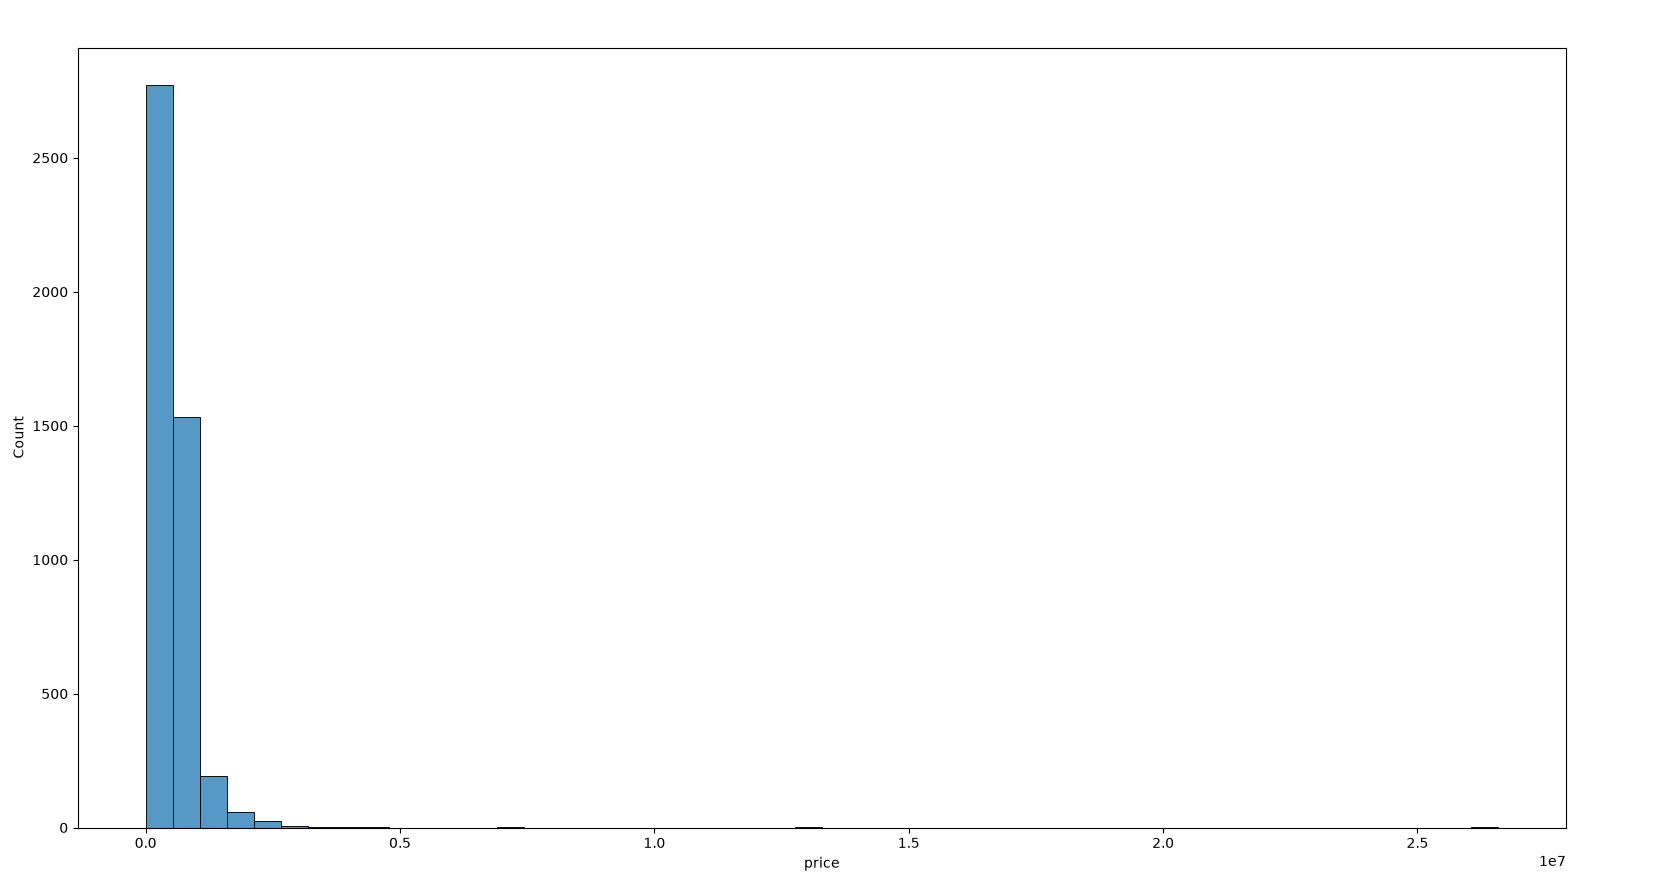
\includegraphics[width=1\textwidth]{prices.png}
\end{center}
\pagebreak
There's a couple of clear outliers in the data, a house that costs a whopping $\$26{,}000{,}000$, as well as some others between that, while most of the houses lie in the $\$300k-400k$ Dollar range.
This graph unfortunately does not show all the houses with a price of \$0. There's a total of 49 properties with a listed price of \$0; this heavily skews the standard-deviation and hurts the model performance.
For the zero-price values, we can simply remove these rows, since \$0 does not reflect the actual value of the property (a low bid, or perhaps the house was given away).
For the extreme values, we can take the logarithm of them, which compresses the right-skewed tail and reduces the influence of the outliers. The resulting $R^2$ score of the regression model is 0.805 for the training data, and 0.774 for the testing data.
I also calculated an RMSE of 0.269 and a MAE of 0.165 in the logarithmic scale. For the actual Dollar value, I got a MAE of $\$110{,}188.80$ and an RMSE of $\$486{,}176.91$.
	This may look like a significant difference at first, but it makes sense: RMSE penalizes larger errors more heavily than MAE does, and the largest values in our dataset are $>10\times$ the average. We can't do much about this gap without removing the extreme values,
	which I can't really justify, as they do actually represent real house prices, unlike the zero-price values.
	I also took a look at the other features present in the data, there's a specific feature that stood out to me; the \texttt{yr\_renivated} feature. Whenever a house has not been renovated, this column is zeroed out.
	This feature is supposed to express the "effective age" of the house, so zeroing out the value is going to mess up the model. What I can do us split this up into 3 different features, \texttt{was\_renovated}: a boolean value representing whether the house has been renovated,
	\texttt{effective\_year}: integer value that is calculated as \texttt{yr\_renovated} if it has been renovated, or \texttt{yr\_built} if it hasn't been renovated, \texttt{age\_at\_sale}: represents the age it is at the time it is sold.
	This does slightly increase our column count, (from 136 to a 139) but considering that our column count is already so high, and this addition is barely anything, I'm letting slide.
	After this pre-processing, we get a $R^2$ score (after cross validation) of 0.789, MAE of $\$110{,}479.7$ and a RMSE of $\$487{,}987$, it increases test scoring slightly, and error stays about the same.
	Considering everything, these will be our benchmarks.
	\\\\
	I found an excellent research paper written in the Jorunal of Research Innovation and Technologie\cite{Housing-ML}. It specifically talks about predicting house prices with machine learning, which is exactly the problem I'm trying to solve.
	In their reasearch results, the Extra Tree algorithm performed best each time, with Random Forest and Gradient Boosting usually landing in second and third respectively. The best option here would probably be the Extra Tree algorithm,
	but since we haven't covered that algorithm in the course, I went with the Random Forest algorithm and the Gradient Boost algorithm.
	The $R^2$ of the Random Forest algorithm was never much worse than the extra tree one ($0.97$ vs. $0.99$), so I think it should suffice.
	\\\\
	Unlike Linear Regression, tree based models like random forests and XGBoost don't require scaled input, and don't benefit from one-hot method, in fact,
	it actively hurts it in this case; with an extra 117 columns in our data, a lot of them being sparse, each individual tree split has a shrinking chance of picking a useful one.
	I used \emph{TargetEncoding} for the \texttt{city} and \texttt{statezip} features: each catagory becomes a single number, the mean target value associated with that category,
	so a city becomes one informative numeric columns instead of dozens of sparse boolean ones. The only risk involved with this is that the mean is computed from the very rows the models will train on,
	so a categroy could leak information about its own target value back into the feature, particularly for cities with few homes. To avoid this, sickit-learn's \texttt{TargetEncoder} computes the encoding using k-fold cross-fitting internally:
	each row's encoded value is computed from the other folds only, never from itself. I used 5 internal folds with a fixed random state for reproducibility.
	\\\\
	The inital training (no hyperparameter tuning) of the models produced an $R^2$ of about 0.764 for the XGBoost model, and 0.774 for the Random Forest model.
	The hyperparameters that I chose for the Random Forest model were: \texttt{max\_depth}, \texttt{min\_sample\_leaf} and \texttt{max\_features}, \texttt{n\_estimators} would've been useless to tune for, as more trees is always better, it never overfits the model. \\
	\texttt{min\_samples\_split} is also a reduntent paramater to tune, I'm  already tuning for the \texttt{min\_sample\_leaf}, they both control when a node stops splitting, and including both in the search usually just doubles the search space and doesn't meaningfully change the results.
	I also skipped the \texttt{criterion} parameter, it usually explodes the time to compute, and doesnt really change our results by a meaningful amount.
	I gave each parameter here 4 values to pick from, so thats $4\times4\times4 = 64\text{ combos } \times 5\text{ folds} = 320$ cross validations, my personal timing (on a 12th Gen Intel Core i7-1260P) of one Random Forest cross validation took 19.23 seconds to compute,
	this would give us $19.23 \times 320 = 1.6h$, which is why I'm going with a RandomizedSearchCV with an $\texttt{n\_iter} = 20$.
	\\\\
	For the XGBoost model, I'm picking \texttt{learning\_rate}, \texttt{n\_estimators}, \texttt{max\_depth}, \texttt{min\_child\_weight}, \texttt{sub\_sample}, \texttt{colsample\_bytree} and \texttt{reg\_lambda}
	Unlike Random Forest, XGBoost builds its trees sequentially, each one correcting the errors of the previous ones, so it is far more prone to overfitting if left unchecked; this is why most of the parameters I picked exist specifically to regularize it.
	\texttt{learning\_rate} and \texttt{n\_estimators} are tuned together, as they trade off directly: a lower learning rate needs more trees to reach the same fit, so I searched them jointly rather than in isolation.
	\texttt{max\_depth} is kept much lower here (3--8) than for the Random Forest (up to 30), since boosting is already an additive process, deep trees at every step compound on top of each other and overfit quickly.
	\texttt{min\_child\_weight} plays a similar role to Random Forest's \texttt{min\_samples\_leaf}, it stops a split if it would leave too little data behind. \texttt{subsample} and \texttt{colsample\_bytree} randomly leave out rows and columns for each tree, which mirrors what \texttt{max\_features} does for the Random Forest, decorrelating the trees from each other.
	Finally, \texttt{reg\_lambda} adds an $L2$ penalty directly on the leaf weights, which is a regularization option Random Forest doesn't have, and is particularly relevant given how easily boosting overfits.

	I did not tune \texttt{gamma} or \texttt{reg\_alpha}: \texttt{gamma} overlaps heavily with \texttt{min\_child\_weight} in what it controls, and \texttt{reg\_alpha} (an $L1$ penalty) mainly helps when many features are weakly relevant, which is less of a concern here since target encoding already leaves us with a small, dense, informative set of features rather than dozens of sparse one-hot columns.
	I did not use early stopping either; it needs a held-out validation set for each fit, which does not fit cleanly inside a cross-validated pipeline, so I tuned \texttt{n\_estimators} directly in the grid instead as a simpler substitute.
	One Cross Validation on the XGBoost (on the same hardware), took 235.38 seconds, which is a lot more than the Random Forest.
	This grid has $3\times4\times4\times3\times3\times3\times3 = 3{,}888$ combinations,
	I did not tune \texttt{gamma} or \texttt{reg\_alpha}: \texttt{gamma} overlaps heavily with \texttt{min\_child\_weight} in what it controls, and \texttt{reg\_alpha} (an $L1$ penalty) mainly helps when many features are weakly relevant, which is less of a concern here since target encoding already leaves us with a small, dense, informative set of features rather than dozens of sparse one-hot columns.
	I did not use early stopping either; it needs a held-out validation set for each fit, which does not fit cleanly inside a cross-validated pipeline, so I tuned \texttt{n\_estimators} directly in the grid instead as a simpler substitute.
	This grid has $3\times4\times4\times3\times3\times3\times3 = 3{,}888$ combinations, which is far too many to search exhaustively; a single XGBoost cross-validation took roughly X seconds to compute on the same machine as before, so I again used a \texttt{RandomizedSearchCV}, this time with $\texttt{n\_iter}=30$.
	Which is far too many to search exhaustively; a single XGBoost cross-validation took roughly 235.38 seconds to compute on the same machine as before, which gives a total time of $3{,}888 \times 235.38 = 10.59$ days of computing. So I again used a \texttt{RandomizedSearchCV}, this time with $\texttt{n\_iter}=30$.




\section{Results}
\section{Conclusion}
\section{Future Work}
\begin{thebibliography}{9}

	\bibitem{Housing-ML}
	Ogundeji, G. A., Pitts, D. D. A., Sun, Y., \& Ghafoor, M. (2024). \emph{Predicting UK Housing Price using Machine Learning Algorithms.} J. Res. Innov. Technol., 3(1), 67-85. \textcolor{RoyalBlue}{\url{https://doi.org/10.57017/jorit.v3.1(5).05}}
\end{thebibliography}

\end{document}
